%----------------------------------------------------------------------------------------
%	PACKAGES AND OTHER DOCUMENT CONFIGURATIONS
%----------------------------------------------------------------------------------------

\documentclass[titlepage]{article}

\usepackage{fancyhdr} % Required for custom headers
\usepackage{lastpage} % Required to determine the last page for the footer
\usepackage{extramarks} % Required for headers and footers
\usepackage{graphicx} % Required to insert images
\usepackage{pdflscape} % Allow us to make certain pages in landscape orientation
\usepackage{amsmath} % Allow multiple line equations
\usepackage{amssymb}
\usepackage{scrextend}
\usepackage{xcolor}
\usepackage{listings} 
\usepackage{dirtree}
\usepackage{hyperref}
\usepackage[numbers]{natbib} 

% Margins
\topmargin=-0.45in
\evensidemargin=0in
\oddsidemargin=0in
\textwidth=6.5in
\textheight=9.0in
\headsep=0.25in 

\linespread{1.1} % Line spacing

% Set up the header and footer
\pagestyle{fancy}
\lhead{}
\chead{Chassis Controller Manual}
\rhead{}
\lfoot{\lastxmark} % Bottom left footer
\cfoot{} % Bottom center footer
\rfoot{Page\ \thepage\ of\ \pageref{LastPage}} % Bottom right footer
\renewcommand\headrulewidth{0.4pt} % Size of the header rule
\renewcommand\footrulewidth{0.4pt} % Size of the footer rule

\setlength\parindent{0pt} % Removes all indentation from paragraphs

%----------------------------------------------------------------------------------------
%	DOCUMENT STRUCTURE COMMANDS
%----------------------------------------------------------------------------------------

\setcounter{secnumdepth}{0} % Removes default section numbers
   
%----------------------------------------------------------------------------------------
%	NAME AND CLASS SECTION
%----------------------------------------------------------------------------------------

\newcommand{\Title}{Python Implementation Manual} % Assignment title
\newcommand{\DueDate}{30 December 2018} % Due date
\newcommand{\Class}{Chassis Controller} % Course/class
\newcommand{\AuthorName}{QUT Motorsport} 

%----------------------------------------------------------------------------------------
%	TITLE PAGE
%----------------------------------------------------------------------------------------

\title{
\vspace{2in}
\textmd{\huge\textbf{\Class}}\\
\textmd{{\Title}}\\
\vspace{3in}
\textmd{{\AuthorName}}
}
\author{}

%----------------------------------------------------------------------------------------

\begin{document}

\maketitle

\tableofcontents

\clearpage

%----------------------------------------------------------------------------------------
%	INSTALLATION
%----------------------------------------------------------------------------------------
\section{Installation}

%----------------------------------------------------------------------------------------
%	INSTALLATION
%----------------------------------------------------------------------------------------

This program can be run on any Linux distribution that supports SocketCAN. This may change in the future when specific RaspberryPi code is added. It's recommended that this program in run on a virtual machine to avoid polluting a daily workstation. 
\\
\\
The initial step is to clone the GitHub repository with the following command:
\begin{lstlisting}[language=bash]
git clone https://github.com/pedrohva/ChassisController.git
\end{lstlisting}
For prototyping, a virtual CAN is setup containing three buses. This emulates the three physical CAN buses present in the vehicle. This virtual network can be set up with the following commands:
\begin{lstlisting}[language=bash]
cd ChassisController
sudo ./setup_CAN.sh
\end{lstlisting}
It's necessary to run the script with sudo in order to install the can-utils package and to set up the interfaces used by the virtual CAN buses.
\newline
To test if the  network was successfully created, use the commands:
\begin{lstlisting}[language=bash]
candump -L vcan0
cansend vcan0 123#DEADBEEF
\end{lstlisting}
Figure \ref{fig:can-test} shows the different IDs and messages that can be sent through the network. 
\begin{figure} [!ht]
	\centering
	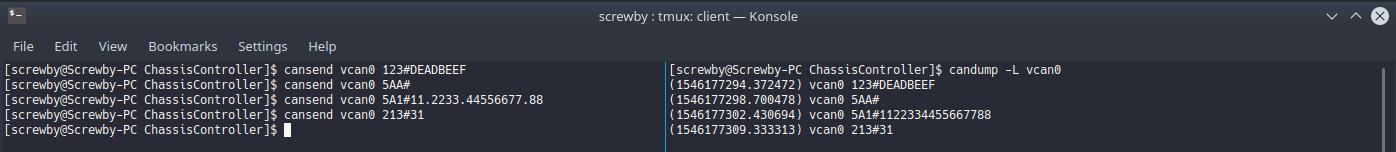
\includegraphics[width=1\textwidth]{manual-src/images/can_test} 
	\caption{Communicating using the virtual CAN through the terminal}
	\label{fig:can-test} 
\end{figure}
\\
To remove the CAN ports, the script can be run again with the argument -r:
\begin{lstlisting}[language=bash]
sudo ./setup_CAN.sh -r
\end{lstlisting}
The Chassis Controller can then be run on its normal operation mode by executing the Python script \emph{normal-operation.py}.
\begin{lstlisting}[language=bash]
python3 normal-operation.py
\end{lstlisting}
It might be useful to use a Python virtual environment. More information about setting it up can be found \href{https://docs.python.org/3.7/tutorial/venv.html}{here}.

\clearpage

\end{document}
